\documentclass[tikz,border=10pt]{standalone}
\usetikzlibrary{arrows.meta,positioning,decorations.pathreplacing,fit,backgrounds}
\usepackage{xcolor}
\pagecolor{white}
\begin{document}
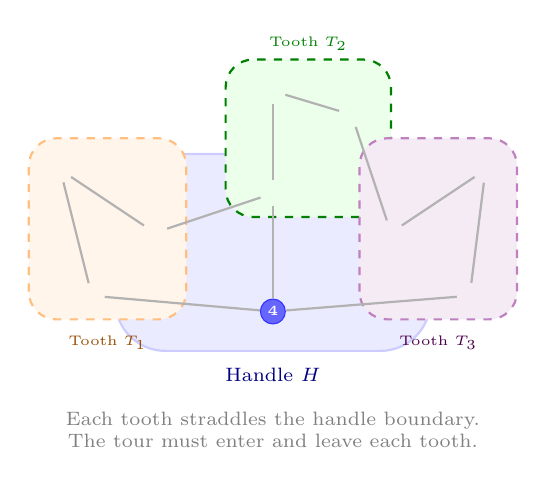
\begin{tikzpicture}[
  city/.style={circle, draw=blue!80, fill=blue!60, inner sep=0pt,
               minimum size=9pt, font=\tiny\bfseries, text=white},
  edge/.style={thick, gray!60},
]
  % Handle cities
  \node[city] (h1) at (0, 1)   {1};
  \node[city] (h2) at (1.5, 1.5) {2};
  \node[city] (h3) at (3, 1)   {3};
  \node[city] (h4) at (1.5, 0)   {4};

  % Tooth 1 cities (straddles handle boundary)
  \node[city, fill=orange!70] (t1a) at (-1.2, 1.8) {a};
  \node[city, fill=orange!70] (t1b) at (-0.8, 0.2) {b};

  % Tooth 2 cities
  \node[city, fill=green!60!black] (t2a) at (1.5, 2.8) {c};
  \node[city, fill=green!60!black] (t2b) at (2.5, 2.5) {d};

  % Tooth 3 cities
  \node[city, fill=violet!70] (t3a) at (4.2, 1.8) {e};
  \node[city, fill=violet!70] (t3b) at (4.0, 0.2) {f};

  % Handle region
  \begin{scope}[on background layer]
    \draw[blue!20, fill=blue!8, thick, rounded corners=18pt]
      (-0.5, -0.5) rectangle (3.5, 2.0);
  \end{scope}
  \node[font=\scriptsize, blue!50!black] at (1.5, -0.8) {Handle $H$};

  % Tooth regions
  \draw[orange!50, fill=orange!8, thick, dashed, rounded corners=10pt]
    (-1.6, -0.1) rectangle (0.4, 2.2);
  \node[font=\tiny, orange!60!black] at (-0.6, -0.4) {Tooth $T_1$};

  \draw[green!50!black, fill=green!8, thick, dashed, rounded corners=10pt]
    (0.9, 1.2) rectangle (3.0, 3.2);
  \node[font=\tiny, green!50!black] at (1.95, 3.4) {Tooth $T_2$};

  \draw[violet!50, fill=violet!8, thick, dashed, rounded corners=10pt]
    (2.6, -0.1) rectangle (4.6, 2.2);
  \node[font=\tiny, violet!60!black] at (3.6, -0.4) {Tooth $T_3$};

  % Tour edges (showing the pattern)
  \draw[edge] (t1a) -- (h1);
  \draw[edge] (h1) -- (h2);
  \draw[edge] (h2) -- (t2a);
  \draw[edge] (t2a) -- (t2b);
  \draw[edge] (t2b) -- (h3);
  \draw[edge] (h3) -- (t3a);
  \draw[edge] (t3a) -- (t3b);
  \draw[edge] (t3b) -- (h4);
  \draw[edge] (h4) -- (t1b);
  \draw[edge] (t1b) -- (t1a);
  \draw[edge] (h2) -- (h4);

  % Annotation
  \node[font=\scriptsize, align=center, text=gray] at (1.5, -1.5)
    {Each tooth straddles the handle boundary.\\The tour must enter and leave each tooth.};
\end{tikzpicture}
\end{document}
